\chapter{继承与多态概述}

\cppsign{} 首先是一门面向对象的语言,对象是 C++ 程序的基本构建单元。类层次结构用于表达软件系统不同部分之间的关系与交互、定义并实现组件之间的接口、以及组织数据与代码。虽然本书并不是一本教授 C++ 语法的教材,本章的目标是为读者提供与类与继承相关的 C++ 语言特性所需的足够背景知识,便于在后续章节中使用。因此我们不会穷举关于“如何使用类”的全部工具,而是聚焦于本书后面将反复使用的概念与语言结构。

本章将讨论如下主题:

\begin{itemize}
\item 什么是类,它在 C++ 中扮演什么角色?
\item 什么是类层次结构,C++ 如何使用继承?
\item 什么是运行时多态,它在 C++ 中如何实现与使用?
\end{itemize}

\section{类与对象}

面向对象编程是一种通过把算法(操作)与其处理的数据组合到一起形成 \textbf{对象} 来组织程序的方式。大多数面向对象语言(包括 C++)都是基于类的。一个 \textbf{类} 是对象的定义——它描述算法和数据、其组织形式以及与其它类的关系。对象是类的一个具体实例,也就是变量。对象有地址,即内存中的一个位置。类是用户自定义类型。通常情况下,可以根据一个类的定义实例化任意多个对象(某些类会限制可创建对象的数量,但那是例外而非常态)。

在 C++ 中,类中包含的数据被组织为一组数据成员(变量),它们可以是不同的类型。算法以函数的形式实现——即类的方法(成员函数)。虽然语言并不强制要求类的数据成员必须与其方法的实现相关,但当数据被很好地封装且方法对外部数据的交互有限时,这往往是良好设计的迹象。

所谓 \textbf{封装} 是 C++ 类的核心概念——语言允许我们控制哪些数据成员和方法是公有的(对类外可见),哪些是内部实现(私有)。一个良好设计的类通常拥有大部分(甚至全部)私有数据成员,而其公有方法仅用于表达类对外的公共接口——换言之“这个类能做什么”。公共接口像一份契约——类的设计者承诺该类提供某些特性与操作。类的私有数据与私有方法属于实现细节,只要公共接口(契约)仍然成立,实现就可以改变。下面的类示例表示一个有理数,并通过其公共接口提供自增(复合加)操作:

\begin{code}
class Rational { 
public:
  Rational& operator+=(const Rational& rhs);
};
\end{code}

一个良好设计的类不会在公共接口中暴露多余的实现细节。实现不是契约的一部分,尽管接口文档可能对实现施加一些约束。比如如果我们承诺所有的有理数都已\emph{约分}(分子与分母没有公因子),那么加法操作就应该包含约分步骤。这是私有成员函数的一个良好用途——多个操作的实现都需要调用它,但类的使用者无需显式调用,因为对外暴露的任意有理数都已经是最简形式:

\begin{code}
class Rational {
  public:
  Rational& operator+=(const Rational& rhs); private:
  long n_; // numerator
  long d_; // denominator
  void  reduce();
};
Rational& Rational::operator+=(const Rational& rhs) {
  n_ = n_*rhs.d_ + rhs.n_*d_;
  d_ = d_*rhs.d_; reduce();
  return *this;
}
Rational a, b; a += b;
\end{code}

类的方法对数据成员有特殊访问权限——它们可以访问类的私有数据。注意这里类与对象的区分——\texttt{operator+=()} 是 \texttt{Rational} 类的成员函数,并在对象 \texttt{a} 上调用。然而它也能访问对象 \texttt{b} 的私有数据,因为 \texttt{a} 与 \texttt{b} 属于同一个类。如果成员函数在引用类成员时直接使用名字而不添加限定符,那么访问的是当前调用对象的对应成员(我们也可以显式写作 \texttt{this-\textgreater{}n\_}、\texttt{this-\textgreater{}d\_})。访问同一类的另一个对象的成员需要该对象的指针或引用,但除此之外没有其它限制;若从一个非成员函数中访问私有成员则不被允许。

顺便提及,C++ 也支持 C 风格的 \emph{struct}。但在 C++ 中,struct 不再局限于仅仅是一组数据成员——它同样可以拥有方法、public / private 访问控制以及类具备的其它任何特性。从语言角度看,class 与 struct 的唯一差异是默认访问权限——class 中成员默认是 private,而 struct 中默认是 public。除此之外,使用 struct 或 class 只是约定问题——传统上 struct 用于 C 风格的结构体(在 C 中也合法)以及“几乎”C 风格的结构体(例如只额外提供一个构造函数)。当然这界限并不精确,取决于项目或团队的编码风格。

除了已经看到的普通(非静态)成员,C++ 还支持静态数据与静态方法。静态成员函数与普通的非成员函数很相似——它并不在某个具体对象上调用,获得任何对象访问的唯一途径是其参数。然而和非成员函数不同,静态成员函数仍保有访问类私有数据的特权。

类本身已经是将算法与其处理的数据组合(封装)并限制部分数据访问的一种有用方式。然而 C++ 中最强大的面向对象特性是继承及其形成的类层次结构。

\section{继承与类层次结构}

在 C++ 中,类层次结构有两个作用:一方面它们让我们能够表达对象之间的关系;另一方面它们允许我们从简单类型组合出更复杂的类型。这两个用途都通过继承实现。

继承是 C++ 使用类与对象的核心概念。继承允许我们以已有类为基础扩展定义新类。派生类从基类继承而来,它以某种形式包含基类的全部数据与算法,并增加自身内容。在 C++ 中,需要区分两种主要的继承形式——public 继承与 private 继承。

public 继承继承的是类的公共接口。它也继承实现——基类的数据成员成为派生类的一部分。但接口的继承是 public 继承的关键特征——派生类的公共接口中包含了基类的公共成员函数。

记住公共接口像一份契约——我们向类的使用者承诺它支持某些操作、维护某些不变式并遵守特定约束。通过 public 继承,我们让派生类也受该契约约束(再加上派生类可能新增的公开接口)。因为派生类也遵守基类接口契约,所以在代码中凡是需要基类的地方都可以使用派生类实例——虽然我们在那一位置不能使用任何新增的扩展接口(因为调用方只“知道”基类),但基类接口及其约束必须依然有效。

这常以 \emph{is-a 原则} 表达——一个派生类的实例同时也是一个基类实例。不过,在 C++ 中理解 \emph{is-a} 关系有时并不直观。举例:正方形是长方形吗?如果是,我们可以从 \texttt{Rectangle} 派生 \texttt{Square}:

\begin{code}
class Rectangle {
  public:
  double Length() const { return length_; }
  double Width()  const { return width_; }
  ...
  private:
  double l_;
  double w_;
};
class Square : public Rectangle {
  ...
};
\end{code}

立刻出现不协调之处——派生类拥有两个表示尺寸的数据成员,但它其实只需要一个,必须强制保持二者相等。看似不难——\texttt{Rectangle} 的接口允许任意正的长与宽,而 \texttt{Square} 再附加额外限制。但问题更糟——\texttt{Rectangle} 的契约允许用户让长宽不相等,而且可以相当明确:

\begin{code}
class Rectangle {
  public:
  void Scale(double sl, double sw) {
     // Scale the dimensions
    length_ *= sl;
    width_  *= sw;
  }
  ...
};
\end{code}

现在我们有一个公有方法允许改变矩形的长宽比。与其它公有方法一样,它被派生类继承,所以 \texttt{Square} 也有它。事实上,通过 public 继承,我们断言一个 \texttt{Square} 对象在任何需要 \texttt{Rectangle} 的地方都可使用,而调用方甚至无需知道它其实是正方形。显然这是我们无法兑现的承诺——当客户端试图修改正方形的长宽比时,我们做不到。我们可以忽略调用或在运行时报错,但无论哪种都违反了基类契约。唯一的解决:在 C++ 里,正方形不是长方形。同理,长方形通常也不是正方形——\texttt{Square} 接口可能提供额外保证,若将 \texttt{Rectangle} 派生自 \texttt{Square} 我们也无法维护。

类似地,如果“鸟”接口包含“会飞”,那么企鹅在 C++ 中就不是鸟。正确设计通常是引入一个更抽象的基类 \texttt{Bird},它不做至少某个派生类无法保证的承诺(比如 \texttt{Bird} 不保证会飞)。然后创建中间基类如 \texttt{FlyingBird} 与 \texttt{FlightlessBird},再从它们派生更具体的 \texttt{Eagle} 或 \texttt{Penguin}。关键在于:企鹅是否是鸟取决于我们如何定义“鸟”,即 \texttt{Bird} 类公共接口包含什么。

由于 public 继承意味着 \emph{is-a} 关系,语言允许在同一层次结构中引用与指针在不同类之间进行多种转换。首先,从派生类指针到基类指针的转换是隐式的(引用同理):

\begin{code}
class Base { ... };
class Derived : public Base { ... };
Derived* d = new Derived;
Base* b = d;    // 隐式转换
\end{code}

该转换总是合法的,因为派生对象同时也是一个基类对象。反向转换可以,但必须显式:

\begin{code}
Base* b = new Derived;     // *b 实际上是 Derived
Derived* d = b; // 不编译,不能隐式转为 Derived*
Derived* d1 =
     static_cast<Derived*>(b);    // 显式转换
\end{code}

之所以不允许隐式,是因为只有当基类指针实际指向一个派生对象时该转换才有效(否则行为未定义)。程序员必须通过 \cii{static_cast} 明确断言——基于程序逻辑、先前测试或其它手段——此转换有效。如果不确定,还有更安全的方式(下一节介绍)。

注意,基类与派生类指针之间的静态(或隐式)转换并不像看起来那样简单。任何对象的第一个基类总与派生对象地址相同,但多重继承时会复杂:

\begin{code}
class Base1 { ... };
class Base2 { ... };
class Derived : public Base1, public Base2 { ... };
\end{code}

大多数编译器会先布局基类,再放派生类的数据成员:
\begin{figure}[H]
\centering
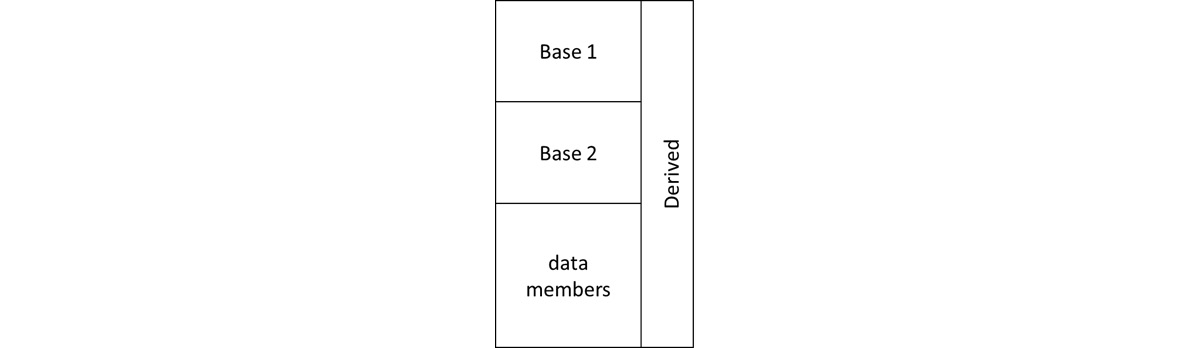
\includegraphics[keepaspectratio]{./image/Figure_1.1_B19262.jpg}
\caption{派生类的一种可能内存布局}
\label{fig1}
\end{figure}

从图 \ref{fig1} 可见,基类与派生类之间的指针转换通常涉及偏移计算。示例:

\begin{code}
// Example 01_cast.C
Derived d;
Derived* p = &d;
std::cout << "Derived: " << (void*)(p) <<
  " Base1: " << (void*)(static_cast<Base1*>(p)) <<
  " Base2: " << (void*)(static_cast<Base2*>(p)) <<
  std::endl;
\end{code}

程序输出类似:

\begin{code}
Derived: 0x7f97e550 Base1: 0x7f97e550 Base2: 0x7f97e560
\end{code}

可以看到 \texttt{Base1} 对象与 \texttt{Derived} 地址相同,而 \texttt{Base2} 有一个偏移(本例 16 字节)。看起来转换就是简单计算:如果你有一个 \texttt{Derived} 指针想转到 \texttt{Base2},加 16 即可。基类之间的偏移在编译期已知,编译器知道其布局。指针加偏移通常由硬件支持(现代 CPU 都支持),无需额外加法指令。似乎并不难。

那么如果指针是 \ci{null} 呢?指针值是 0。如果应用同样的“转换”,你得到 \texttt{16 (0x10)},此时你的空指针检查失效:

\begin{code}
void f(Base2* p) {
  if (p != nullptr) do_work(*p);
}
Derived* p = nullptr;
f(p); // 会尝试解引用 0x10 吗?
\end{code}

显然这很糟,所以我们可以假定 \ci{null} 保持为 \ci{null}。确实如此:

\begin{code}
Derived* p = nullptr;
std::cout << "Derived: " << (void*)(p) <<
  " Base1: " << (void*)(static_cast<Base1*>(p)) <<
  " Base2: " << (void*)(static_cast<Base2*>(p)) <<
  std::endl;
\end{code}

输出:

\begin{code}
Derived: 0x0 Base1: 0x0 Base2: 0x0
\end{code}

这是唯一可行的实现方式,但意味着一个从 \texttt{Derived*} 到 \texttt{Base*} 的简单隐式转换内部隐藏了一个对 \ci{null} 的条件分支。

另一种继承是 \textbf{private 继承}。私有继承时,派生类不会扩展基类的公共接口——基类方法在派生类中都变为私有。任何公共接口必须由派生类重新自定义(白纸起步)。并不假定派生类对象可以当作基类对象使用。派生类获得的是实现细节——可以使用基类的方法与数据成员实现自己的算法。因此常说 private 继承表达的是 \emph{has-a} 关系——派生对象内部包含一个基类实例。

私有继承后派生类与其基类的关系类似“类与其数据成员”的关系。后者实现技巧称为 \textbf{组合}(composition)——一个对象由任意数量的其它对象组成,后者作为数据成员。在没有特殊理由时应优先选择组合而非私有继承。那么什么时候用私有继承?有几种可能。第一,可以在派生类内用 \cii{using} 声明重新公开基类的某个 public 成员函数:

\begin{code}
class Container : private std::vector<int> {
  public:
  using std::vector<int>::size;
  ...
};
\end{code}

这在少数场景有用,但等价于一个内联转发函数:

\begin{code}
class Container {
  private:
  std::vector<int> v_;
  public:
  size_t size() const { return v_.size(); }
  ...
};
\end{code}

第二,可以在派生类成员函数内部把派生对象指针或引用转换为基类指针或引用;组合情况下等价于取数据成员地址。到此为止尚无充分理由使用私有继承,确实通常建议首选组合。但接下来两个理由更重要,任意一个都可能成为使用私有继承的动机。

其一与对象大小有关。常见存在“只提供方法、不含数据成员”的基类。此类没有自身数据,理应不占内存。但在 C++ 中它们必须拥有非零大小,这是因为语言要求任意两个不同对象/变量有不同唯一地址。通常若两个变量顺序声明,后者地址是前一个地址加上其大小:

\begin{code}
int x;     // 地址 0xffff0000,大小 4
int y;     // 地址 0xffff0004
\end{code}

为避免单独处理 0 大小对象,C++ 规定空对象大小为 1。如果这样的对象作为类的数据成员,它至少占 1 字节(后续成员的对齐可能增加此值)。这是浪费的内存,不会真正使用。而若空类作为基类使用,则没有要求其基类子对象必须有非零大小。整个派生对象必须非零,但派生对象地址、其第一个基类子对象地址以及其第一个数据成员地址都可以相同。因此 C++ 允许对空基类不分配额外内存,即使 \texttt{sizeof()} 对该类返回 1。虽然该“空基类优化”不是强制的,但大多数现代编译器都实现了:

\begin{code}
class Empty {
  public:
  void useful_function();
};
class Derived : private Empty {
  int i;
};    // sizeof(Derived) == 4
class Composed {
  int i;
  Empty e;
};    // sizeof(Composed) == 8
\end{code}

如果我们需要大量创建派生对象,节省的内存可能很可观。

第二个使用私有继承的理由与虚函数相关,下一节解释。

\section{多态与虚函数}

前面讨论 public 继承时我们提到,派生对象可以在任何需要基类对象的地方使用。虽然如此,很多时候我们仍希望知道对象的真实类型——即它被构造时的类型:

\begin{code}
Derived d;
Base& b = d;
...
b.some_method(); // b 实际上是 Derived 对象
\end{code}

\texttt{some\_method()} 属于 \texttt{Base} 公共接口,对 \texttt{Derived} 也必须有效。但在基类契约允许的灵活空间内,它可以“做不同的事情”。仍以鸟类层次为例:\texttt{FlyingBird} 可以假设存在一个 \texttt{fly()} 方法,所有从其派生的特定鸟类都必须支持飞行。但鹰与秃鹫的飞行方式不同,因此 \texttt{Eagle} 与 \texttt{Vulture} 中 \texttt{fly()} 的实现可以不同。对任意 \texttt{FlyingBird} 对象操作的代码可以调用 \texttt{fly()},而结果取决于对象真实类型。

该功能在 C++ 中由虚函数实现。虚的公共成员函数必须在基类中声明:

\begin{code}
class FlyingBird : public Bird {
  public:
  virtual void fly(double speed, double direction) {
    ... move the bird at the specified speed
        in the given direction ...
  }
  ...
};
\end{code}

派生类继承该函数的声明与实现。声明及其契约必须被遵守。如果该实现满足派生类需求则无需再做任何事;否则可以覆盖(override)基类实现:

\begin{code}
class Vulture : public FlyingBird {
  public:
  virtual void fly(double speed, double direction) {
    ... move the bird but accumulate
        exhaustion if too fast ...
  }
};
\end{code}

注意,派生类中覆盖基类虚函数时使用 \texttt{virtual} 关键字是可选的,没有语义影响(稍后会看到在某些风格中建议省略)。

调用虚函数时,C++ 运行时系统必须确定对象的真实类型。通常这一信息在编译期未知,只能在运行时判定:

\begin{code}
void hunt(FlyingBird& b) {
  b.fly(...);    // 可能是 Vulture 或 Eagle
  ...
};
Eagle e;
hunt(e);   // hunt() 内 b 实为 Eagle
           // 调用 FlyingBird::fly()
Vulture v;
hunt(v);   // b 实为 Vulture
           // 调用 Vulture::fly()
\end{code}

这种技术:一段代码操作一批基类对象并调用相同方法,而实际运行结果依对象真实类型而异,被称为 \textbf{运行时多态},支持该技术的对象被称为 \textbf{多态对象}。在 C++ 中,多态对象必须至少有一个虚函数,并且只有接口中通过虚函数实现(部分或全部实现)的部分才具备多态行为。

由此可知,虚函数声明与其覆盖实现必须一致——程序员在基类对象接口上调用函数,而实际运行的是派生类版本,仅当两者参数与返回类型一致时才可能。一个例外:若基类虚函数返回某类型的指针或引用,则覆盖允许返回该类型的派生类型的指针或引用(\textbf{协变返回类型})。

一个非常常见的多态层次特例是:基类没有一个“良好”默认实现。例如所有会飞的鸟都会飞,但它们的速度不同,没有理由在基类选一个速度作为默认。在 C++ 中我们可以拒绝在基类提供实现。

这样的函数称为 \textbf{纯虚函数}(pure virtual),包含纯虚函数的基类称为 \textbf{抽象类}:

\begin{code}
class FlyingBird {
  public:
  virtual void fly(...) = 0;     // 纯虚函数
};
\end{code}

抽象类只定义接口;由具体派生类实现。如果基类包含纯虚函数,程序中每个可被实例化的派生类都必须提供实现。换言之不能直接创建基类对象(派生类也可继续是抽象类,此时仍不能直接实例化,需再派生)。不过我们可以拥有指向基类对象的指针或引用——它们实际指向某个派生类型,但通过基类接口进行操作。

关于语法:覆盖虚函数时不必重复 \texttt{virtual}。若基类已经声明某名字与参数列表的虚函数,派生类同名同参函数自动为虚并覆盖基类。如果参数不同,则不会覆盖而是隐藏(shadow)基类同名函数,可能导致微妙 Bug:程序员意欲覆盖却没有正确匹配声明:

\begin{code}
class Eagle : public FlyingBird {
  public:
  void fly(int speed, double direction);
};
\end{code}

此处参数类型略有不同。\texttt{Eagle::fly()} 仍是虚的,但并未覆盖 \texttt{FlyingBird::fly()}。若后者为纯虚函数,编译器会因未实现而报错;若其有默认实现,则该 Bug 不会被编译器检测。C++11 提供 \texttt{override} 关键字帮助捕捉此类问题:

\begin{code}
class Eagle : public FlyingBird {
  public:
  void fly(int speed, double direction) override;
};
\end{code}

此时即使省略 \texttt{virtual} 也没关系;若 \texttt{FlyingBird} 中没有可被覆盖的虚函数,此代码无法编译。

也可以用 \texttt{final} 禁止进一步覆盖:

\begin{code}
class Eagle : public FlyingBird {
  public:
  // 所有 Eagle 飞行方式一致,BaldEagle / GoldenEagle 不能再改。
  void fly(int speed, double direction) final;
};
\end{code}

使用 \texttt{final} 很少见:很少设计要求完全禁止后续自定义。\texttt{final} 也可用于整个类,表示不可再派生,同样罕见。

那么覆盖时是否应再次写 \texttt{virtual}? 这是风格问题,但风格影响可读性与可维护性。推荐实践:

\begin{itemize}
\item 任何不覆盖基类函数的新虚函数必须写 \texttt{virtual}(包括无基类的类中的函数,以及派生类新增的虚函数)。
\item 其它覆盖函数不再写 \texttt{virtual},全部使用 \texttt{override}(例外:下一条)。
\item 最终覆盖(不允许再覆盖)使用 \texttt{final},且不再写 \texttt{override}。
\end{itemize}

这样有两点好处。其一:清晰——看到 \texttt{virtual} 就知道它不覆盖任何基类;看到 \texttt{override} 则必然是覆盖(否则不编译);看到 \texttt{final} 则同样是覆盖且是最后一次。其二:维护性——层次维护的大问题是“基类脆弱性”:你写了一组类,后来有人给基类函数加了一个参数,结果所有派生类函数不再覆盖,永远不被调用。始终使用 \texttt{override} 可以避免。

虚函数最常见的使用是结合 public 继承——由于每个派生对象也是基类对象(\emph{is-a}),程序可以把一组派生对象当作同类集合处理,而虚函数覆盖确保每个对象得到正确处理:

\begin{code}
void MakeLoudBoom(std::vector<FlyingBird*> birds)
  for (auto bird : birds) {
    bird->fly(...);   // 同一调用,结果不同
  }
}
\end{code}

但虚函数也可用于私有继承。用法不那么直观(且远少见)——毕竟私有继承的基类是“不可访问基类”(inaccessible base),尝试将派生指针转为基类失败。然而有一个上下文允许该转换:在派生类成员函数内部。以下展示如何让私有继承基类中的虚函数调用分派到派生:

\begin{code}
class Base {
  public:
  virtual void f() {
      std::cout << "Base::f()" << std::endl;
    }
  void g() { f(); }
};
class Derived : private Base {
  public:
  virtual void f() {
    std::cout << "Derived::f()" << std::endl;
  }
  void h() { g(); }
};
Derived d;
d.h(); // 输出 "Derived::f()"
\end{code}

\texttt{Base} 的公有方法在 \texttt{Derived} 中变为私有,因此我们不能直接调用。但可以在 \texttt{Derived} 的其它成员函数(如公有的 \texttt{h()})内部调用。我们当然可以直接在 \texttt{h()} 调用 \texttt{f()},但那无法证明任何事情——没人会惊讶 \texttt{Derived::h()} 调用 \texttt{Derived::f()}。

相反我们调用从 \texttt{Base} 继承的 \texttt{Base::g()}。在该函数内部我们处于 \texttt{Base} 上下文——其函数体可能在 \texttt{Derived} 实现前很久就写好、编译好。然而此处虚函数分派仍正常工作,调用 \texttt{Derived::f()},就像 public 继承一样。

上一节我们建议除非有理由,否则优先组合而非私有继承。这里的虚函数行为无法用组合轻易实现;若需要此行为,只能使用私有继承。

一个含虚函数的类必须在每个对象中编码其动态类型——这是在将指针转换为基类指针并丢失静态类型信息后在运行时知道对象真实类型的唯一手段。类型信息不是免费的:它占空间——多态对象总比相同数据成员但无虚函数的对象更大(通常多一个指针大小)。

额外大小与虚函数数量无关——只要有一个虚函数就需要类型信息。回想:基类指针可以转换为派生指针,但前提是我们知道正确的派生类型。使用 \cii{static_cast} 无法验证假设。对于非多态类(无虚函数),一旦丢失原始类型就无法恢复。但对多态对象,其类型编码在对象里,因此必须有办法利用该信息检查我们关于派生类型的假设是否成立。确实存在:\cii{dynamic_cast}:

\begin{code}
class Base { ... };
class Derived : public Base { ... };
Base* b1 = new Derived;     // 实际是 Derived
Base* b2 = new Base;   // 不是 Derived
Derived* d1 = dynamic_cast<Derived*>(b1);  // 成功
Derived* d2 = dynamic_cast<Derived*>(b2);  // d2 == nullptr
\end{code}

\cii{dynamic_cast} 不会告诉我们对象真实类型是什么;它让我们问一个问题——真实类型是 \texttt{Derived} 吗?如果猜对,转换成功并返回派生对象指针;否则返回 \ci{null}。\cii{dynamic_cast} 也能用于引用,差异仅在于——没有“空引用”:函数若返回引用必须指向有效对象,因此当请求类型不匹配真实类型时,只能抛出异常。

对性能敏感代码,需要关注 \cii{dynamic_cast} 的运行时成本。直觉可能认为虚函数调用与 \cii{dynamic_cast} 开销相近:两者都类似“这个 \texttt{Base} 指针其实是 \texttt{Derived} 吗?”的判定。简单基准表明并非如此:

\begin{code}
// Example 02_dynamic_cast.C
class Base {
  protected:
  int i = 0;
  public:
  virtual ~Base() {}
  virtual int f() { return ++i; }
};
class Derived : public Base {
  int f() override { return --i; }
};
Derived* p = new Derived;
// 测量 p->f() 的运行时间
// 测量 dynamic_cast<Derived*>(p) 的运行时间
\end{code}

基准可能显示(绝对值依硬件)虚调用约 1ns,而 \cii{dynamic_cast} 约 5~10ns。为何 \cii{dynamic_cast} 更贵?我们需要更多关于层次结构的背景(见下一节多重继承)。

\section{多重继承}

在 C++ 中,类可以同时从多个基类派生。回到鸟的例子:会飞的鸟彼此有很多共性,同时它们与其它会飞的动物(比如蝙蝠、昆虫)共享“飞行能力”。因飞行不限于鸟,我们可以把处理飞行的数据与算法抽离到独立基类。但鹰无疑也是一种鸟。若我们希望同时表达这两个关系,可以让 \texttt{Eagle} 继承两个基类:

\begin{code}
class Eagle : public Bird, public FlyingAnimal { ... };
\end{code}

此处两个继承均为 public,意味着派生类继承两个接口并需履行两份契约。若两个接口中都有同名方法会怎样?如果该方法不是虚的,则在派生类上调用会二义性而无法编译;如果该方法是虚的且派生类提供覆盖,则不再二义,因为调用派生实现。\texttt{Eagle} 现在既是 \texttt{Bird} 又是 \texttt{FlyingAnimal}:

\begin{code}
Eagle* e = new Eagle;
Bird* b = e;
FlyingAnimal* f = e;
\end{code}

两种向上转换都允许,反向转换需显式 static 或 dynamic cast。还有一个有趣转换——如果我们有一个 \texttt{FlyingAnimal} 指针,它同时也是一个 \texttt{Bird},能否从一个基转换到另一个基?可以,用 \cii{dynamic_cast}:

\begin{code}
Bird* b = new Eagle;   // 同时也是 FlyingAnimal
FlyingAnimal* f = dynamic_cast<FlyingAnimal*>(b);
\end{code}

在该上下文中 \cii{dynamic_cast}有时称为 \textbf{交叉转换}(\emph{cross-cast})——不是沿层次“向上/向下”而是“横向”在不同分支基类之间。

交叉转换也是 \cii{dynamic_cast}高成本的重要原因。虽然其最常用途是从 \texttt{Base*} 转到 \texttt{Derived*} 验证是否真是派生对象,但它也可能在同一派生对象的不同基之间转换。这是更难的问题。如果只是检查一个基对象是否真是某个特定派生类型,编译器此时知道 \texttt{Derived} 类型(\cii{dynamic_cast} 不能用于不完整类型),也就知道该派生的所有基类,检查是否其中之一很简单。但跨层次转换时,编译器仅知道两个基类:此时代码可能还不存在一个组合两者的派生类,它会在未来编写。编译器必须现在就生成正确代码:运行时遍历所有可能同时继承二者的派生类,判断当前对象是否其中之一(实际实现更高效,但目标相同)。

现实中这类开销通常不必要,因为大多数 \cii{dynamic_cast}确实只是做基到特定派生的判定。在很多场合这点开销无关紧要;但若需要更好性能,则没有办法让 \cii{dynamic_cast}更快。若想快速判断一个多态对象是否为给定类型,必须使用虚函数并(不幸地)维护一个所有可能类型(或感兴趣类型)的列表:

\begin{code}
enum type_t { typeBase, typeDerived1, typeDerived2 };
class Base {
  virtual type_t type() const { return typeBase; }
};
class Derived1 : public Base {
  type_t type() const override { return typeDerived1; }
};
鈥? // 省略其它派生
void process_derived1(Derived1* p);
void do_work(Base* p) {
  if (p->type() == typeDerived1) {
    process_derived1(static_cast<Derived1*>(p));
  }
}
\end{code}

多重继承在 C++ 中常被诟病。大量反对意见来自早期编译器对其实现差、效率低的年代。现代编译器下这已不再是主要顾虑。人们还说多重继承让层次更难理解与推理;更准确地说,设计一个良好且准确反映不同属性关系的多重继承层次更难,而糟糕的层次确实难以理解。

这些担忧主要适用于使用 public 继承的层次。多重继承也可以是私有的。相比单一私有继承,使用多重私有继承代替组合更加缺乏理由。不过空基类优化可以同时应用于多个空基类,若适用,仍是一个合理动机:

\begin{code}
class Empty1 {};
class Empty2 {};
class Derived : private Empty1, private Empty2 {
  int i;
};   // sizeof(Derived) == 4
class Composed {
  int i;
  Empty1 e1;
  Empty2 e2;
};   // sizeof(Composed) == 8
\end{code}

当派生类表示一个组合了多个互不重叠属性的系统时,多重继承尤其有效。后续本书在探讨各种设计模式及其 C++ 表示时会遇到这种情况。

\section{总结}

本章虽不是类与对象的完整指南或参考,但介绍并解释了理解本书其余章节示例所需的概念。我们的关注点在于用 C++ 表达设计模式,因此本章聚焦于正确使用类与继承,尤其注意通过哪些 C++ 特性表达不同组件之间的关系与交互——设计模式正是通过这些特性构建出的结构。

下一章将以类似方式介绍 C++ 模板相关知识,为理解后续章节奠定基础。

\section{问题}

\begin{itemize}
\item 对象在 C++ 中的重要性是什么?
\item public 继承表达什么关系?private 继承表达什么关系?什么是多态对象?
\item \cii{dynamic_cast}与 \cii{static_cast} 的区别是什么?为何 \cii{dynamic_cast}更昂贵?
\end{itemize}

\section{延伸阅读}

\begin{itemize}
\item \emph{Deciphering Object-Oriented Programming with C++}: \url{https://www.packtpub.com/product/deciphering-object-oriented-programming-with-c/9781804613900}
\item \emph{Software Architecture with C++}: \url{https://www.packtpub.com/product/software-architecture-with-c/9781838554590}
\item \emph{C++ Fundamentals}: \url{https://www.packtpub.com/product/c-fundamentals}
\item \emph{C++ Data Structures and Algorithms}:\url{ https://www.packtpub.com/product/c-data-structures-and-algorithm-design-principles}
\item \emph{Mastering C++ Programming}: \url{https://www.packtpub.com/product/mastering-c-programming}
\item \emph{Beginning C++ Programming}: \url{https://www.packtpub.com/product/beginning-c-programming}
\end{itemize}
%\chapter{An Introduction to Inheritance and Polymorphism}
%
%\textbf{C++} is, first and foremost, an object-oriented language, and objects are the fundamental building blocks of a C++ program. Class hierarchies are used to express relationships and interactions between different parts of a software system, define and implement interfaces between components, and organize data and code. While this isn't a book for teaching C++, the aim of this chapter is to give the reader enough knowledge about C++ language features as they relate to classes and inheritance, which will be used in later chapters. To that end, we won't attempt to completely describe the C++ tools for working with classes but introduce the concepts and language constructs that will be used throughout this book.
%
%The following topics will be covered in this chapter:
%
%\begin{itemize}
%\item
%  What are classes and what is their role in C++?
%\item
%  What are class hierarchies and how does C++ use inheritance?
%\item
%  What is runtime polymorphism and how is it used in C++?
%\end{itemize}
%
%\section{Classes and objects}
%
%Object-oriented programming is a way to structure a program by combining the algorithms and the data that the algorithms operate on into single entities called \textbf{objects}. Most object-oriented languages, including C++, are class-based. A \textbf{class} is a definition of an object---it describes the algorithms and the data, its format, and its relations to other classes. An object is a concrete instantiation of a class, that is, a variable. An object has an address, which is a location in memory. A class is a user-defined type. In general, any number of objects can be instantiated from the definition provided by the class (some classes limit the number of objects that can be created, but this is an exception, not the norm).
%
%In C++, the data contained in a class is organized as a collection of data members, or variables, of different types. The algorithms are implemented as functions---the methods of the class. While there's no language requirement that the data members of a class should be somehow relevant to the implementation of its methods, it's one of the signs of good design when the data is well encapsulated in the classes, and the methods have limited interaction with external data.
%
%This concept of \textbf{encapsulation} is central to the classes in C++---the language allows us to control which data members and methods are public---visible outside of the class, and which are internal---private to the class. A well-designed class has mostly, or only, private data members, and the only public methods are those needed to express the public interface of the class---in other words, what the class does. This public interface is like a contract---the class designer promises that this class provides certain features and operations. The private data and methods of the class are part of the implementation, and they can be changed as long as the public interface, the contract we've committed to, remains valid. For example, the following class represents a rational number and supports the increment operation, as exposed by its public interface:
%
%\begin{code}
%class Rational { public:
%  Rational& operator+=(const Rational& rhs);
%};
%\end{code}
%
%A well-designed class doesn't expose any more of the implementation details than it has to through its public interface. The implementation isn't part of the contract, although the documented interface may impose some restrictions on it. For example, if we promise that all rational numbers don't contain any common multipliers in the numerator and denomination, the addition should include the step of canceling them. That would be a good use of a private member function---the implementation of several other operations will need to call it, but the client of the class never needs to call it because every rational number is already reduced to its lowest terms before it's exposed to the callers:
%
%\begin{code}
%class Rational {
%  public:
%  Rational& operator+=(const Rational& rhs); private:
%  long n_; // numerator
%  long d_; // denominator
%  void  reduce();
%};
%Rational& Rational::operator+=(const Rational& rhs) {
%  n_ = n_*rhs.d_ + rhs.n_*d_;
%  d_ = d_*rhs.d_; reduce();
%  return *this;
%}
%Rational a, b; a += b;
%\end{code}
%
%The class methods have special access to the data members---they can access the private data of the class. Note the distinction between the class and the object here---\texttt{operator+=()} is a method of the \texttt{Rational} class and is invoked on the object, \texttt{a}. However, it has access to the private data of the \texttt{b} object as well, because \texttt{a} and \texttt{b} are objects of the same class. If a member function references a class member by name without any additional qualifiers, then it's accessing a member of the same class it's invoked on (we can make it explicit by writing \texttt{this-\textgreater{}n\_} and \texttt{this-\textgreater{}d\_}). Accessing members of another object of the same class requires a pointer or a reference to that object, but is otherwise not restricted, as would have been the case if we tried to access a private data member from a non-member function.
%
%By the way, C++ also supports C-style structs. But in C++, a struct isn't limited to just an aggregate of data members---it can have methods, public and private access modifiers, and anything else classes have. From a language point of view, the only difference between a class and a struct is the default access---in a class, all members and methods are private by default, while in a struct they're public. Beyond that, the use of structs instead of classes is a matter of convention---traditionally, structs are used for C-style structs (structs that would be legal in C) as well as \emph{almost} C-style structs, for example, a struct with only a constructor added. Of course, this boundary isn't precise and is a matter of coding styles and practices in each project or team.
%
%In addition to the methods and data members we've seen, C++ also supports static data and methods. A static method is very similar to a regular non-member function---it isn't invoked on any particular object, and the only way it can get access to an object of any type is through its arguments. However, unlike a non-member function, a static method retains its privileged access to the private data of the class.
%
%Classes by themselves are a useful way to group together (encapsulate) the algorithms and the data they operate on and to limit access to some data. However, the most powerful object-oriented features of C++ are inheritance and the resulting class hierarchies.
%
%\section{Inheritance and class hierarchies}
%
%Class hierarchies in C++ serve a dual purpose. On the one hand, they allow us to express relations between objects. On the other hand, they let us compose more complex types from simpler ones. Both uses are accomplished through inheritance.
%
%The concept of inheritance is central to the C++ use of classes and objects. Inheritance allows us to define new classes as extensions of existing ones. When a derived class is inherited from the base class, it contains, in some form, all of the data and the algorithms that were in the base class, and it adds some of its own. In C++, it's important to distinguish between two primary types of inheritance---public and private.
%
%Public inheritance inherits the public interface of the class. It also inherits the implementation---the data members of the base class are also a part of the derived class. But the inheritance of the interface is what distinguishes public inheritance---the derived class has, as a part of its public interface, the public member functions of the base class.
%
%Remember that the public interface is like a contract---we promise to the clients of the class that it supports certain operations, maintains some invariants, and obeys the specified restrictions. By publicly inheriting from the base class, we bind the derived class to the same contract (plus any extensions of the contract, should we decide to define additional public interfaces). Because the derived class also respects the interface contract of the base class, we could use a derived class in any place in the code where a base class is expected---we would not be able to use any of the extensions to the interface (the code expects the base class, we don't know about any extensions at that point), but the base class interface and its restrictions have to be valid.
%
%This is often expressed as the \emph{is-a principle}---an instance of a derived class is also an instance of the base class. However, the way we interpret the \emph{is-a} relationship in C++ isn't exactly intuitive. For example, is a square a rectangle? If it is, then we can derive the \texttt{Square} class from the \texttt{Rectangle} class:
%
%\begin{code}
%class Rectangle {
%  public:
%  double Length() const { return length_; }
%  double Width() const { return width_; }
%  ...
%  private:
%  double l_;
%  double w_;
%};
%class Square : public Rectangle {
%  ...
%};
%\end{code}
%
%Right away, there's something that doesn't seem right---the derived class has two data members for dimensions, but it really needs only one. We would have to somehow enforce that they're always the same. This doesn't seem so bad---the \texttt{Rectangle} class has the interface that allows for any positive values of length and width, and the \texttt{Square} imposes additional restrictions. But it's worse than that---the \texttt{Rectangle} class has a contract that allows the user to make the dimensions different. This can be quite explicit:
%
%\begin{code}
%class Rectangle {
%  public:
%  void Scale(double sl, double sw) {
%     // Scale the dimensions
%    length_ *= sl;
%    width_ *= sw;
%  }
%  ...
%};
%\end{code}
%
%Now, we have a public method that allows us to distort the rectangle, altering its aspect ratio. As with any other public method, it's inherited by the derived classes, so now the \texttt{Square} class has it too. In fact, by using public inheritance, we assert that a \texttt{Square} object can be used anywhere a \texttt{Rectangle} object is used, without even knowing that it's really a \texttt{Square}. Clearly, this is a promise we can't keep---when the client of our class hierarchy tries to change the aspect ratio of a square, we can't do it. We could ignore the call or report an error at runtime. Either way, we've violated the contract provided by the base class. There's only one solution---in C++, a square isn't a rectangle. Note that a rectangle is usually not a square, either---the contract provided by the \texttt{Square} interface could contain any number of guarantees that we can't maintain if we derive the \texttt{Rectangle} class from \texttt{Square}.
%
%Similarly, a penguin isn't a bird in C++ if the bird interface includes flying. The correct design for such cases usually includes a more abstract base class, \texttt{Bird}, that doesn't make any promises that at least one derived class can't keep (for example, a \texttt{Bird} object doesn't make a guarantee that it can fly). Then, we create intermediate-based classes, such as \texttt{FlyingBird} and \texttt{FlightlessBird}, that are derived from the common base class and serve as base classes for the more specific classes such as \texttt{Eagle} or \texttt{Penguin}. The important lesson here is that whether or not a penguin is a bird in C++ depends on how we define what a bird is, or, in C++ terms, what the public interface of the \texttt{Bird} class is.
%
%Because the public inheritance implies the \emph{is-a} relationship, the language allows a wide range of conversions between references and pointers to different classes in the same hierarchy. First of all, a conversion from a pointer to a derived class into a pointer to the base class is implicit (this is the same for references):
%
%\begin{code}
%class Base { ... };
%class Derived : public Base { ... };
%Derived* d = new Derived;
%Base* b = d;    // Implicit conversion
%\end{code}
%
%This conversion is always valid because an instance of the derived class is also an instance of the base class. The inverse conversion is possible but has to be made explicit:
%
%\begin{code}
%Base* b = new Derived;     // *b is really Derived
%Derived* d = b; // Does not compile, not implicit Derived*
%Derived* d1 =
%     static_cast<Derived*>(b);    // Explicit conversion
%\end{code}
%
%The reason this conversion isn't implicit is that it's valid only if the base class pointer really points to a derived object (otherwise, the behavior is undefined). The programmer, therefore, must explicitly assert, using the static cast, that somehow, through the logic of the program or a prior test or by some other means, it's known that this conversion is valid. If you aren't sure that the conversion is valid, there's a safer way to try it without causing undefined behavior; we'll learn about this in the next section.
%
%Note that the static (or implicit) conversion between pointers to base and derived classes is not quite as straightforward as you might think. The first base of any object always has the same address as the derived object itself, but then it gets more complicated. There is generally no standard requirement on the memory layout of derived classes with multiple bases:
%
%\begin{code}
%class Base1 { ... };
%class Base2 { ... };
%class Derived : public Base1, public Base2 { ... };
%\end{code}
%
%Most compilers will lay out the base classes first, then the data members of the derived class:
%
%\pandocbounded{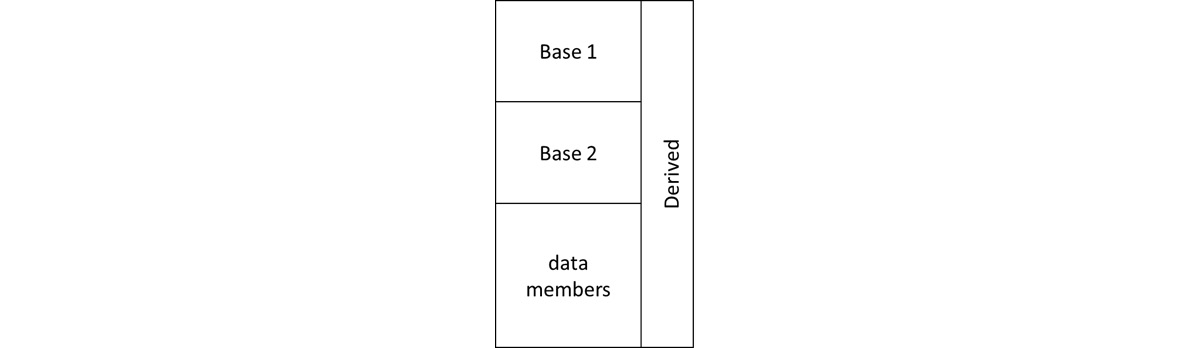
\includegraphics[keepaspectratio]{./image/Figure_1.1_B19262.jpg}}
%
%Figure 1.1 -- Possible memory layout of a derived class
%
%From \emph{Figure 1.1}, it is evident that pointer conversion between the base and derived classes generally involves offset calculations. We can easily see this in an example:
%
%\begin{code}
%// Example 01_cast.C
%Derived d;
%Derived* p = &d;
%std::cout << "Derived: " << (void*)(p) <<
%  " Base1: " << (void*)(static_cast<Base1*>(p)) <<
%  " Base2: " << (void*)(static_cast<Base2*>(p)) <<
%  std::endl;
%\end{code}
%
%The program prints something like this:
%
%\begin{code}
%Derived: 0x7f97e550 Base1: 0x7f97e550 Base2: 0x7f97e560
%\end{code}
%
%You can see that the \texttt{Base1} object is located at the same address as the \texttt{Derived} object, and \texttt{Base2} starts with an offset (16 bytes, in our case). Seems like the cast is an easy calculation: If you have a pointer to \texttt{Derived} and you want to cast to \texttt{Base2}, add 16. The offsets between base classes are known at compile time, and the compiler knows the layout it is using. Pointer offset calculations are usually implemented in hardware (all modern CPUs support them and do not require a separate addition instruction). This doesn't sound so hard at all.
%
%Now, what do you do if the pointer is \ci{null}? The pointer has a value of 0. If you apply the same \emph{conversion}, you get \texttt{16\ (0x10)}, and now your check for \ci{null} fails:
%
%\begin{code}
%void f(Base2* p) {
%  if (p != nullptr) do_work(*p);
%}
%Derived* p = nullptr;
%f(p); // Will it try to dereference 0x10?
%\end{code}
%
%Obviously, this would be very bad, so we can assume that \ci{null} pointers remain so. Indeed, they do:
%
%\begin{code}
%Derived* p = nullptr;
%std::cout << "Derived: " << (void*)(p) <<
%  " Base1: " << (void*)(static_cast<Base1*>(p)) <<
%  " Base2: " << (void*)(static_cast<Base2*>(p)) <<
%  std::endl;
%\end{code}
%
%This prints the same values for all pointers:
%
%\begin{code}
%Derived: 0x0 Base1: 0x0 Base2: 0x0
%\end{code}
%
%This is the only way to do casts, but it implies that a simple implicit cast from \texttt{Derived*} to \texttt{Base*} hides inside a conditional computation with a \ci{null} pointer check.
%
%The other kind of inheritance in C++ is \textbf{private inheritance}. When inheriting privately, the derived classes don't extend the public interface of the base class---all base class methods become private in the derived class. Any public interface has to be created by the derived class, starting from a clean slate. There's no assumption that an object of the derived class can be used in place of an object of the base class. What the derived class does get from the base class is the implementation details---both the methods and the data members can be used by the derived class to implement its own algorithms. It's said, therefore, that private inheritance implements a \emph{has-a} relationship---the derived object has an instance of the base class contained inside of it.
%
%The relation of the privately derived class to its base class is, therefore, similar to that of the relationship of a class to its data members. The latter implementation technique is known as \textbf{composition}---an object is composed of any number of other objects, which are all used as its data members. In the absence of any reason to do otherwise, the composition should be preferred to private inheritance. What, then, might be the reasons to use private inheritance? There are several possibilities. First of all, it's possible, within the derived class, to re-expose one of the public member functions of the base class with the help of a \texttt{using} declaration:
%
%\begin{code}
%class Container : private std::vector<int> {
%  public:
%  using std::vector<int>::size;
%  ...
%};
%\end{code}
%
%This can be useful in rare cases, but it's also equivalent to an inline forwarding function:
%
%\begin{code}
%class Container {
%  private:
%  std::vector<int> v_;
%  public:
%  size_t size() const { return v_.size(); }
%  ...
%};
%\end{code}
%
%Second, a pointer or reference to a derived object can be converted into a pointer or reference to the base object, but only inside a member function of the derived class. Again, the equivalent functionality for composition is provided by taking the address of a data member. So far, we haven't seen a good reason to use private inheritance, and indeed, the common advice is to prefer composition. But the next two reasons are more significant, and either one could be motivation enough to use private inheritance.
%
%One good reason to use private inheritance has to do with the size of the composed or derived objects. It isn't uncommon to have base classes that provide only methods but no data members. Such classes have no data of their own and, therefore, should not occupy any memory. But in C++, they have to be given a non-zero size. This has to do with the requirement that any two different objects or variables have different and unique addresses. Typically, if we have two variables declared one after the other, the address of the second one is the address of the first one, plus the size of the first one:
%
%\begin{code}
%int x;     // Created at address 0xffff0000, size is 4
%int y;     // Created at address 0xffff0004
%\end{code}
%
%To avoid the need to handle zero-sized objects differently, C++ assigns an empty object the size of one. If such an object is used as a data member of a class, it occupies at least 1 byte (the alignment requirements for the next data member may increase this value). This is wasted memory; it'll never be used for anything. On the other hand, if an empty class is used as a base class, there's no requirement that the base part of an object must have a non-zero size. The entire object of the derived class must have a non-zero size, but the address of a derived object, its base object, and its first data member can all be at the same address. Therefore, it's legal in C++ to allocate no memory for an empty base class, even though \texttt{sizeof()} returns 1 for this class. While legal, such empty base class optimization isn't required and is considered an optimization. Nonetheless, most modern compilers do this optimization:
%
%\begin{code}
%class Empty {
%  public:
%  void useful_function();
%};
%class Derived : private Empty {
%  int i;
%};    // sizeof(Derived) == 4
%class Composed {
%  int i;
%  Empty e;
%};    // sizeof(Composed) == 8
%\end{code}
%
%If we create many derived objects, the memory saved by the empty base optimization can be significant.
%
%The second reason to possibly use private inheritance has to do with virtual functions, and this will be explained in the next section.
%
%\section{Polymorphism and virtual functions}
%
%When we discussed public inheritance earlier, we mentioned that a derived object can be used in any place where a base object is expected. Even with this requirement, it's often useful to know what the actual type of the object is---in other words, what type the object was created as:
%
%\begin{code}
%Derived d;
%Base& b = d;
%...
%b.some_method(); // b is really a Derived object
%\end{code}
%
%\texttt{some\_method()} is a part of the public interface of the \texttt{Base} class and has to be valid for the \texttt{Derived} class as well. But, within the flexibility allowed by the contract of the base class interface, it can do something different. As an example, we've already used the avian hierarchy before to represent different birds, in particular, birds that can fly. The \texttt{FlyingBird} class can be assumed to have a \texttt{fly()} method, and every specific bird class derived from it has to support flight. But eagles fly differently from vultures, and so the implementation of the \texttt{fly()} method in the two derived classes, \texttt{Eagle} and \texttt{Vulture}, can be different. Any code that operates on arbitrary \texttt{FlyingBird} objects can call the \texttt{fly()} method, but the results will vary depending on the actual type of the object.
%
%This functionality is implemented in C++ using virtual functions. A virtual public function must be declared in the base class:
%
%\begin{code}
%class FlyingBird : public Bird {
%  public:
%  virtual void fly(double speed, double direction) {
%    ... move the bird at the specified speed
%        in the given direction ...
%  }
%  ...
%};
%\end{code}
%
%A derived class inherits both the declaration and the implementation of this function. The declaration and the contract it provides must be respected. If the implementation meets the needs of the derived class, there's no need to do anything more. But if the derived class needs to change the implementation, it can override the implementation of the base class:
%
%\begin{code}
%class Vulture : public FlyingBird {
%  public:
%  virtual void fly(double speed, double direction) {
%    ... move the bird but accumulate
%        exhaustion if too fast ...
%  }
%};
%\end{code}
%
%Note that the keyword \texttt{virtual}, when used in a derived class for methods that override base class virtual functions, is entirely optional and has no effect; we will see later that there are good reasons to omit that.
%
%When a virtual function is called, the C++ runtime system must determine what the real type of the object is. Usually, this information isn't known at compile time and must be determined at runtime:
%
%\begin{code}
%void hunt(FlyingBird& b) {
%  b.fly(...);    // Could be Vulture or Eagle
%  ...
%};
%Eagle e;
%hunt(e);   // Now b in hunt() is Eagle
%           // FlyingBird::fly() is called
%Vulture v;
%hunt(v);   // Now b in hunt() is Vulture
%           // Vulture::fly() is called
%\end{code}
%
%The programming technique where some code operates on any number of base objects and invokes the same methods, but the results depend on the actual type of these objects, is known as \textbf{runtime polymorphism}, and the objects that support this technique are \textbf{polymorphic}. In C++, polymorphic objects must have at least one virtual function, and only the parts of their interface that use virtual functions for some or all of the implementation are polymorphic.
%
%It should be evident from this explanation that the declaration of the virtual function and its overrides should be identical---the programmer calls the function on a base object, but the version that's implemented in the derived class runs instead. This can happen only if the two functions have identical arguments and return types. One exception is that if a virtual function in the base class returns a pointer or a reference to an object of some type, the override can return a pointer or a reference to an object derived from that type (this is known as \textbf{covariant} \textbf{return types}).
%
%A very common special case of polymorphic hierarchies is one where the base class doesn't have a good \emph{default} implementation of the virtual function. For example, all flying birds fly, but they all fly at different speeds, so there's no reason to select one speed as the default. In C++, we can refuse to provide any implementation for a virtual function in the base class.
%
%Such functions are called \textbf{pure virtual}, and any base class that contains a pure virtual function is known as an \textbf{abstract class}:
%
%\begin{code}
%class FlyingBird {
%  public:
%  virtual void fly(...) = 0;     // Pure virtual function
%};
%\end{code}
%
%An abstract class defines an interface only; it's the job of the concrete derived classes to implement it. If the base class contains a pure virtual function, every derived class that's instantiated in the program must provide an implementation. In other words, an object of a base class can't be created (a derived class could also be an abstract class, but then it cannot be instantiated directly either, we must derive another class from it). We can, however, have a pointer or a reference to an object of a base class---they really point to a derived class, but we can operate on it through the base class interface.
%
%A few notes on the C++ syntax---when overriding a virtual function, it isn't required to repeat the \texttt{virtual} keyword. If the base class declares a virtual function with the same name and arguments, the one in the derived class will always be a virtual function and will override the one from the base class. Note that, if the arguments differ, the derived class function doesn't override anything and instead shadows the name of the base class function. This can lead to subtle bugs where the programmer intended to override a base class function but didn't copy the declaration correctly:
%
%\begin{code}
%class Eagle : public FlyingBird {
%  public:
%  void fly(int speed, double direction);
%};
%\end{code}
%
%Here, the types of the arguments are slightly different. The \texttt{Eagle::fly()} function is also virtual, but it doesn't override \texttt{FlyingBird::fly()}. If the latter is a pure virtual function, the bug will be caught because every pure virtual function must be implemented in a derived class. But if \texttt{FlyingBird::fly()} has the default implementation, then the bug will go undetected by the compiler. C++11 provides a very useful feature that greatly simplifies finding such bugs---any function that's intended to be an override of a base class virtual function can be declared with the \texttt{override} keyword:
%
%\begin{code}
%class Eagle : public FlyingBird {
%  public:
%  void fly(int speed, double direction) override;
%};
%\end{code}
%
%The \texttt{virtual} keyword is still optional, but if the \texttt{FlyingBird} class doesn't have a virtual function that we could be overriding with this declaration, this code won't compile.
%
%It is also possible to prevent the derived classes from overriding a virtual function by declaring it \texttt{final}:
%
%\begin{code}
%class Eagle : public FlyingBird {
%  public:
%  // All Eagles fly the same way, derived classes BaldEagle
%  // and GoldenEagle cannot change this.
%  void fly(int speed, double direction) final;
%};
%\end{code}
%
%Note that the use of the \texttt{final} keyword is rare: it is unusual for the design to require that from this point on, the customizations should be disabled in the hierarchy. The \texttt{final} keyword can also be applied to the entire class: it means that no more classes can be derived from this one. Again, this is a rare situation.
%
%So, should or shouldn't you use the \texttt{virtual} keyword on overrides? This is a matter of style, but the style affects the readability and maintainability of the code. The following is the recommended practice:
%
%\begin{itemize}
%\item
%  Any virtual function that does not override one in the base class must use the \texttt{virtual} keyword. This includes both the functions in classes that have no bases and the functions added in derived classes.
%\item
%  Any other virtual function should not use the \texttt{virtual} keyword. All overrides should use the \texttt{override} keyword, with the following exception, which is also another rule.
%\item
%  A final override must use the \texttt{final} keyword and should not use the \texttt{override} keyword.
%\end{itemize}
%
%There are two advantages to this approach. The first is clarity and readability: if you see \texttt{virtual}, this is a virtual function that does not override anything. If you see \texttt{override}, this must be an override (otherwise the code would not compile). If you see \texttt{final}, this is also an override (again, the code would not compile otherwise) and it's the last such in the hierarchy. The second advantage shows up during code maintenance. One of the greatest problems with maintaining hierarchies is the base class fragility: you write a set of base and derived classes, someone else comes along and adds an argument to the base class function, and suddenly all your derived class functions don't override the base class ones and never get called. With consistent use of the \texttt{override} keyword, this will not happen.
%
%The most common use of virtual functions, by far, is in hierarchies that use public inheritance---since every derived object is also a base object (\emph{is-a} relationship), a program can often operate on a collection of derived objects as if they were all of the same types, and the virtual function overrides ensure that the right processing happens for every object:
%
%\begin{code}
%void MakeLoudBoom(std::vector<FlyingBird*> birds)
%  for (auto bird : birds) {
%    bird->fly(...);   // Same action, different results
%  }
%}
%\end{code}
%
%But virtual functions can also be used with private inheritance. The use is less straightforward (and much less common)---after all, an object that's derived privately can't be accessed through a base class pointer (a private base class is referred to as an \textbf{inaccessible base}, and an attempt to cast a derived class pointer to the base class will fail). However, there's one context in which this cast is permitted, and that's within a member function of the derived class. Here's, then, the way to arrange a virtual function call from a privately inherited base class to the derived one:
%
%\begin{code}
%class Base {
%  public:
%  virtual void f() {
%      std::cout << "Base::f()" << std::endl;
%    }
%  void g() { f(); }
%};
%class Derived : private Base {
%  public:
%  virtual void f() {
%    std::cout << "Derived::f()" << std::endl;
%  }
%  void h() { g(); }
%};
%Derived d;
%d.h(); // Prints "Derived::f()"
%\end{code}
%
%The public methods of the \texttt{Base} class become private in the \texttt{Derived} class, so we can't call them directly. We can, however, call them from another method of the \texttt{Derived} class, such as the public method \texttt{h()}. We can then call \texttt{f()} directly from \texttt{h()}, but that doesn't prove anything---it would come as no surprise if \texttt{Derived::h()} invoked \texttt{Derived::f()}.
%
%Instead, we call the \texttt{Base::g()} function that's inherited from the \texttt{Base} class. Inside that function, we're in the \texttt{Base} class---the body of this function may have been written and compiled long before the \texttt{Derived} class was implemented. And yet, in this context, the virtual function override works correctly and \texttt{Derived::f()} is called, just as it would if the inheritance were public.
%
%In the previous section, we recommended that composition is preferred to private inheritance unless there's a reason to do otherwise. There's no good way to implement similar functionality using composition; so, if the virtual function behavior is desired, private inheritance is the only way to go.
%
%A class with a virtual method has to have its type encoded into every object---this is the only way to know, at runtime, what was the type of the object when it was constructed, after we converted the pointer into a base class pointer and lost any other information about the original type. That type information isn't free; it takes space---a polymorphic object is always larger than an object with the same data members but no virtual methods (usually by the size of a pointer).
%
%The extra size doesn't depend on how many virtual functions the class has---at long as it has one, the type information must be encoded in the object. Now, recall that a pointer to the base class can be converted into a pointer to the derived class, but only if we know the correct type of the derived class. With the static cast, there's no way to test whether our knowledge is correct. For non-polymorphic classes (classes without any virtual functions), there can be no better way; once their original type is lost, there is no way to recover it. But for polymorphic objects, the type is encoded in the object, so there has to be a way to use that information to check whether our assumption is correct about which derived object this really is. Indeed, there is a way. It's provided by the dynamic cast:
%
%\begin{code}
%class Base { ... };
%class Derived : public Base { ... };
%Base* b1 = new Derived;     // Really Derived
%Base* b2 = new Base;   // Not Derived
%Derived* d1 = dynamic_cast<Derived*>(b1);  // Succeeds
%Derived* d2 = dynamic_cast<Derived*>(b2);  // d2 == nullptr
%\end{code}
%
%The dynamic cast doesn't tell us what the real type of the object is; rather, it allows us to ask the question---Is the real type \texttt{Derived}? If our guess at the type is correct, the cast succeeds and returns the pointer to the derived object. If the real type is something else, the cast fails and returns a \ci{null} pointer. The dynamic cast can also be used with references, with similar effects, save one---there's no \emph{null reference}. A function that returns a reference must always return a reference to some valid object. Since the dynamic cast can't return a reference to a valid object if the requested type doesn't match the actual type. The only alternative is to throw an exception.
%
%For performance-conscious code, it is important to be aware of the run-time cost of the dynamic cast. Naively, one might think that a virtual function call and a dynamic cast take about the same time: both boil down to the question -- is this pointer to \texttt{Base} really a pointer to \texttt{Derived}? A simple benchmark shows that this is not so:
%
%\begin{code}
%// Example 02_dynamic_cast.C
%class Base {
%  protected:
%  int i = 0;
%  public:
%  virtual ~Base() {}
%  virtual int f() { return ++i; }
%};
%class Derived : public Base {
%  int f() override { return --i; }
%};
%Derived* p = new Derived;
%// Measure the runtime of p->f();
%// Measure the runtime of dynamic_cast<Derived*>(p);
%\end{code}
%
%The benchmark results should look something like this (the absolute numbers will depend on the hardware): 1 nanosecond for the virtual call, and 5 to 10 nanoseconds for the dynamic cast. Why is the dynamic cast so expensive? We need to learn more about the hierarchies before we can answer this question.
%
%So far, we've limited ourselves to only one base class. While it's much easier to think about class hierarchies if we imagine them as trees, with the base class and the root and branches where multiple classes are derived from the same base, C++ doesn't impose such limitations. Next, we'll learn about inheriting from several base classes at once.
%
%\section{Multiple inheritance}
%
%In C++, a class can be derived from several base classes. Going back to our birds, let's make an observation---while flying birds have a lot in common with each other, they also have something in common with other flying animals, specifically, the ability to fly. Since flight isn't limited to birds, we may want to move the data and the algorithms related to processing flight into a separate base class. But there's also no denying that an eagle is a bird. We could express this relation if we used two base classes to construct the \texttt{Eagle} class:
%
%\begin{code}
%class Eagle : public Bird, public FlyingAnimal { ... };
%\end{code}
%
%In this case, the inheritance from both base classes is public, which means that the derived class inherits both interfaces and must fulfill two separate contracts. What happens if both interfaces define a method with the same name? If this method isn't virtual, then an attempt to invoke it on the derived class is ambiguous, and the program doesn't compile. If the method is virtual and the derived class has an override for it, then there's no ambiguity since the method of the derived class is called. Also, \texttt{Eagle} is now both \texttt{Bird} and \texttt{FlyingAnimal}:
%
%\begin{code}
%Eagle* e = new Eagle;
%Bird* b = e;
%FlyingAnimal* f = e;
%\end{code}
%
%Both conversions from the derived class into the base class pointer are allowed. The reverse conversions must be made explicitly using a static or a dynamic cast. There's another interesting conversion---if we have a pointer to a \texttt{FlyingAnimal} class that's also a \texttt{Bird} class, can we cast from one to the other? Yes, we can with a dynamic cast:
%
%\begin{code}
%Bird* b = new Eagle;   // Also a FlyingAnimal
%FlyingAnimal* f = dynamic_cast<FlyingAnimal*>(b);
%\end{code}
%
%When used in this context, the dynamic cast is sometimes called a \textbf{cross-cast}---we aren't casting up or down the hierarchy (between derived and based classes) but across the hierarchy---between the classes on different branches of the hierarchy tree.
%
%Cross-cast is also mostly responsible for the high runtime cost of the dynamic cast we have seen in the previous section. While the most common use of \texttt{dynamic\_cast} is to cast from \texttt{Base*} to \texttt{Derived*} to verify that a given object is really of the derived class, the cast could also be used to cast between bases of the same derived class. This is a much harder problem. If you just want to check that the base class object is really a derived one, the compiler knows the \texttt{Derived} type at this point (you cannot use the dynamic cast on incomplete types).
%
%Therefore, the compiler knows exactly what base classes this derived type has and can trivially check if yours is one of them. But when casting across the hierarchy, the compiler knows only two base classes: at the time when this code was written, a derived class that combines both may not exist, it will be written later. But the compiler must generate the correct code now. So, the compiler has to generate code that, at run time, digs through all the possible classes that are derived from both base classes to see if yours is one of them (the actual implementation is less straightforward and more efficient than that, but the task to be accomplished remains the same).
%
%In reality, this overhead is often unnecessary because, most of the time, the dynamic cast is indeed used to find out whether the base class pointer really points to a derived object. In many cases, the overhead is not significant. But if better performance is required, there is no way to make the dynamic cast faster. If you want a fast way to check whether a polymorphic object is really of a given type, you have to use virtual functions and, unfortunately, a list of all possible types (or at least all the ones you might be interested in):
%
%\begin{code}
%enum type_t { typeBase, typeDerived1, typeDerived2 };
%class Base {
%  virtual type_t type() const { return typeBase; }
%};
%class Derived1 : public Base {
%  type_t type() const override { return typeDerived1; }
%};
%鈥?
%void process_derived1(Derived1* p);
%void do_work(Base* p) {
%  if (p->type() == typeDerived1) {
%    process_derived1(static_cast<Derived1*>(p));
%  }
%}
%\end{code}
%
%Multiple inheritance is often maligned and disfavored in C++. Much of this advice is outdated and stems from the time when compilers implemented multiple inheritance poorly and inefficiently. Today, with modern compilers, this isn't a concern. It's often said that multiple inheritance makes the class hierarchy harder to understand and reason about. Perhaps it would be more accurate to say that it's harder to design a good multiple inheritance hierarchy that accurately reflects the relations between different properties, and that a poorly designed hierarchy is difficult to understand and reason about.
%
%These concerns mostly apply to hierarchies that use public inheritance. Multiple inheritance can be private as well. There's even less reason to use multiple private inheritance instead of composition than there was to use single private inheritance. However, the empty base optimization can be done on multiple empty base classes and remains a valid reason to use private inheritance, if it applies:
%
%\begin{code}
%class Empty1 {};
%class Empty2 {};
%class Derived : private Empty1, private Empty2 {
%  int i;
%};   // sizeof(Derived) == 4
%class Composed {
%  int i;
%  Empty1 e1;
%  Empty2 e2;
%};   // sizeof(Composed) == 8
%\end{code}
%
%Multiple inheritance can be particularly effective when the derived class represents a system that combines several unrelated, non-overlapping attributes. We'll encounter such cases throughout this book when we explore various design patterns and their C++ representations.
%
%\section{Summary}
%
%While by no means a complete guide or reference to classes and objects, this chapter introduced and explained the concepts you will need to understand the examples and explanations in the rest of this book. As our interest is and will be in representing design patterns in C++, this chapter focused on the proper use of classes and inheritance. We paid particular attention to what relations are expressed through different C++ features---it's through these features we'll express relations and interactions between different components that form a design pattern.
%
%The next chapter will similarly cover knowledge of C++ templates, which will be necessary to understand the subsequent chapters of this book.
%
%\section{Questions}
%
%\begin{itemize}
%\item
%  What is the importance of objects in C++?
%\item
%  Which relation is expressed by public inheritance? Which relation is expressed by private inheritance? What is a polymorphic object?
%\item
%  What is the difference between the dynamic cast and the static cast? Why is the dynamic cast so expensive?
%\end{itemize}
%
%\section{Further reading}
%
%\begin{itemize}
%\item
%  \emph{Deciphering Object-Oriented Programming with} \emph{C++}: https://www.packtpub.com/product/deciphering-object-oriented-programming-with-c/9781804613900
%\item
%  \emph{Software Architecture with} \emph{C++}: https://www.packtpub.com/product/software-architecture-with-c/9781838554590
%\item
%  \emph{C++} \emph{Fundamentals}: https://www.packtpub.com/product/c-fundamentals
%\item
%  \emph{C++ Data Structures and} \emph{Algorithms}: https://www.packtpub.com/product/c-data-structures-and-algorithm-design-principles
%\item
%  \emph{Mastering C++} \emph{Programming}: https://www.packtpub.com/product/mastering-c-programming
%\item
%  \emph{Beginning C++} \emph{Programming}: https://www.packtpub.com/product/beginning-c-programming
%\end{itemize}

